%!TEX root = main.tex

\section{Video tiling}
\label{sec:tiling}

Next, we describe \name's tiling scheme.
% that splits a video into spatial regions each encoded at multiple quality levels, so that the runtime streaming protocol can adapt quality levels according to the users viewport movement.
Our focus is to explain how it splits a video spatially into {\em variable-size} tiles, each encoded at multiple quality levels, such that the runtime streaming protocol could flexibly adapt quality level to optimize user-perceived quality (\S\ref{sec:jnd}).

\mypara{High-level process}
By default, \name temporally splits a video to one-second chunks, and spatially splits each tile into tiles by the following high-level steps (illustrated in Figure~\ref{fig:tiling-steps}).
\begin{packeditemize}
\item {\em Step 1: Fine-grained tiling.} 
\name first splits each chunk into small square tiles with a 12-by-24 grid, which is much finer-grained than most related work (3-by-6 or 4-by-8). Note the tile here consists of the same region of all frames in a one-second chunk.
\item {\em Step 2: Calculating quality-bitrate efficiency.} 
Then for each small tile, \name calculates an ``efficiency'' score that indicates how much user-perceived quality (in PSPNR) could improve by raising the quality level by a small amount. We will present its details next.
\item {\em Step 3: Grouping similar tiles.}
Finally, \name groups the small tiles with similar efficiency score into much fewer large tiles (rectangle but of variable sizes) to increase coding efficiency. 
\end{packeditemize}


\begin{figure}
  \centering
  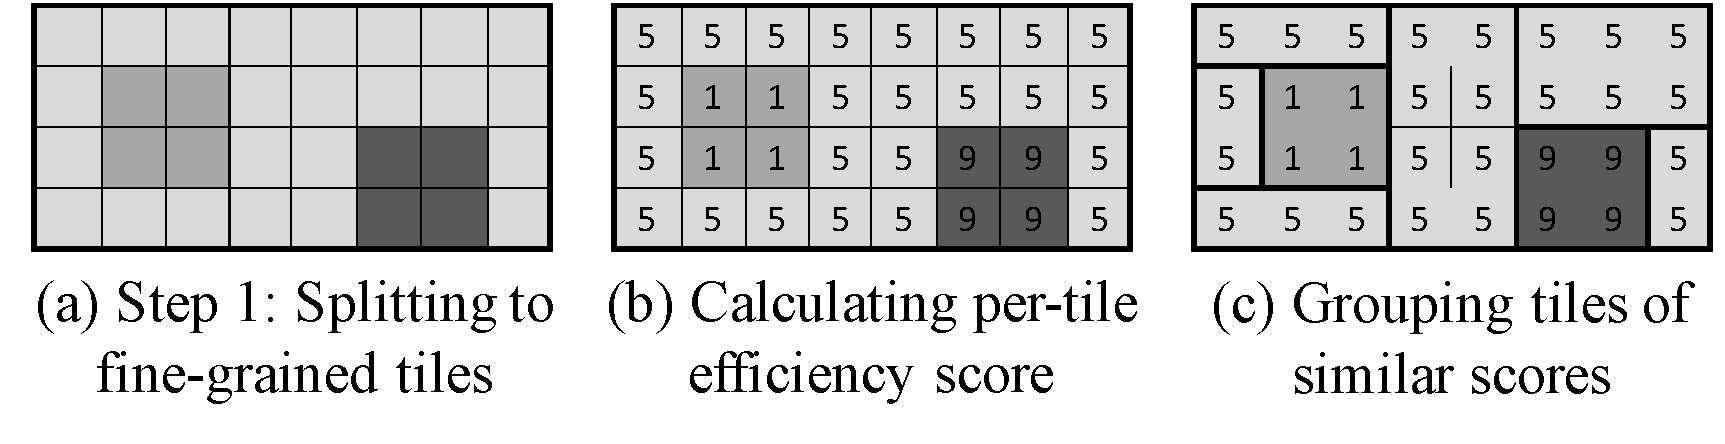
\includegraphics[width=0.5\textwidth]{figures/tiling-steps.pdf}
  \caption{An illustration of tiling steps in \name.}
  \label{fig:tiling-steps}
\end{figure}

\mypara{Calculating per-tile efficiency score}
The key to \name tiling process is the calculation of the efficiency scores. 
For each tile $\Tile$ and quality level $\Quality$ (\eg QP), one can calculate its PSPNR $\PSPNR_\Tile(\Quality)$ based on Equation~\ref{eq:pspnr}.
Formally, the efficiency score represents the gradiate of $\PSPNR_\Tile$ at increasing the quality level by a $\Delta\Quality$.
To simplify its calculation, we approximate this by assuming that $\PSPNR_\Tile$ as a linear function of $\Quality$, so the efficiency score of $\Tile$ is $\Efficiency_\Tile=\frac{\PSPNR_\Tile(\Quality_{high})-\PSPNR_\Tile(\Quality_{low})}{\Quality_{high}-\Quality_{low}}$, where $\Quality_{high}$ and $\Quality_{low}$ denote the values of the highest quality level (QP) and the lowest quality level (QP), respectively.
We found the assumption of linear function of $\PSPNR$ works well, but our solution does not crucially rely on the assumption. 
That is, even if there are inaccuracies in the observations, our solution still provides a lower bound on performance, which can be improved upon by accounting for the inaccuracies. We leave such refinements for future work.

\mypara{Grouping of fine-grained tiles}
The intuition behind grouping small tiles with similar efficiency score (Step 3) is that tiles that have a similarly high (or low) scores are likely to be assigned with similarly high (or low) quality level. 
Therefore, grouping them into large tiles increases video encoding efficiency (\ie smaller size due to reducing redundant information at tile boundaries) at a small cost of perceived quality.
This step can be formulated as a minimum set cover problem that minimizes the score variance in each large tile while maintaining the total number of tiles.
\jc{Guan Yu: add the problem formulation and a short description of the DP solution}


\mypara{Improving tiling with history traces}
Finally, calcuting the PSPNR values based only on video content will lead to inaccuracies, since the three user action-driven factors (\eg viewpoint speed) also heavily influence the JND model and the PSPNR values (\S\ref{sec:jnd}).
Thus, the \name tiling mechanism can benefit from access to some history trace (which has been used by prior work to improve viewport prediction model).
Our empirical analysis has found that by simply ``averaging'' the user actions (\eg mean viewpoint speed) and using these averaged values, we can improve the accuracy of PSPNR and efficiency score calculation. 
This suggests that when most \vrvideo user behaviors are similar (as repeatedly observed in prior work), we can split videos into tiles that help spatial adaptation of quality levels to improve the perceived quality.




